% PQC-LINK progress report 3: the handshake benchmark between two computers.
%
% Continues progress_report_2.tex. Build (any LaTeX with TikZ and pgfplots):
%   latexmk -pdf progress_report_3.tex
% Regenerate the data files from the raw files first:
%   python3 -I prepare_data3.py ~/t10_results data3
% Every number in the results sections comes from data3/numbers3.tex and the generated
% tables and plot data; do not type measurements here.
\documentclass[11pt,a4paper]{article}

\usepackage[margin=2.2cm]{geometry}
\usepackage[T1]{fontenc}
\usepackage{lmodern}
\usepackage{microtype}
\usepackage{xcolor}
\usepackage{booktabs}
\usepackage{tabularx}
\usepackage{array}
\usepackage{caption}
\usepackage{placeins}
\renewcommand{\topfraction}{0.9}\renewcommand{\floatpagefraction}{0.8}
\usepackage{tikz}
\usetikzlibrary{arrows.meta,positioning,fit,backgrounds,calc,shapes.geometric}
\usepackage{pgfplots}
\usepgfplotslibrary{statistics}
\pgfplotsset{compat=1.17}
\usepackage[colorlinks=true,linkcolor=blue!50!black,urlcolor=blue!50!black]{hyperref}

% Generated by prepare_data3.py from the raw files. Do not edit.
\newcommand{\NOneA}{100}
\newcommand{\SlowOneA}{0}
\newcommand{\TlsMedOneA}{0.971}
\newcommand{\TlsPnfOneA}{1.472}
\newcommand{\TotMedOneA}{1.448}
\newcommand{\CCpuMedOneA}{0.319}
\newcommand{\SCpuMedOneA}{0.379}
\newcommand{\NOneB}{100}
\newcommand{\SlowOneB}{2}
\newcommand{\TlsMedOneB}{1.203}
\newcommand{\TlsPnfOneB}{1.696}
\newcommand{\TotMedOneB}{1.687}
\newcommand{\CCpuMedOneB}{0.393}
\newcommand{\SCpuMedOneB}{0.479}
\newcommand{\TlsRatioOne}{1.24}
\newcommand{\TlsDiffOne}{0.231}
\newcommand{\CCpuRatioOne}{1.23}
\newcommand{\CCpuDiffOne}{0.074}
\newcommand{\SCpuRatioOne}{1.26}
\newcommand{\SCpuDiffOne}{0.100}
\newcommand{\RttOne}{0.661/0.822/1.127/0.165 ms}
\newcommand{\DateOne}{2026-10-20}
\newcommand{\ChA}{19{,}520}
\newcommand{\ShA}{15{,}520}
\newcommand{\CtxA}{273}
\newcommand{\CrxA}{757}
\newcommand{\ChB}{27{,}408}
\newcommand{\ShB}{21{,}584}
\newcommand{\CtxB}{1{,}449}
\newcommand{\CrxB}{1{,}845}
\newcommand{\CliCpuModel}{Intel(R) Core(TM) Ultra 9 285H}
\newcommand{\SrvCpuModel}{Intel(R) Core(TM) i7-6700HQ CPU @ 2.60GHz}
\newcommand{\SrvGov}{powersave}
\newcommand{\CliGov}{NA}
\newcommand{\NWarm}{5}
\newcommand{\NTwoA}{100}
\newcommand{\SlowTwoA}{0}
\newcommand{\TlsMedTwoA}{1.142}
\newcommand{\TlsPnfTwoA}{1.634}
\newcommand{\TotMedTwoA}{1.696}
\newcommand{\CCpuMedTwoA}{0.336}
\newcommand{\SCpuMedTwoA}{0.479}
\newcommand{\NTwoB}{100}
\newcommand{\SlowTwoB}{2}
\newcommand{\TlsMedTwoB}{1.305}
\newcommand{\TlsPnfTwoB}{1.890}
\newcommand{\TotMedTwoB}{1.813}
\newcommand{\CCpuMedTwoB}{0.392}
\newcommand{\SCpuMedTwoB}{0.587}
\newcommand{\TlsRatioTwo}{1.14}
\newcommand{\TlsDiffTwo}{0.163}
\newcommand{\CCpuRatioTwo}{1.17}
\newcommand{\CCpuDiffTwo}{0.056}
\newcommand{\SCpuRatioTwo}{1.22}
\newcommand{\SCpuDiffTwo}{0.107}
\newcommand{\RttTwo}{0.695/0.807/0.946/0.094 ms}
\newcommand{\DateTwo}{2026-10-20}
\newcommand{\SameTwoA}{yes}
\newcommand{\SameTwoB}{yes}
\newcommand{\NThreeA}{100}
\newcommand{\SlowThreeA}{0}
\newcommand{\TlsMedThreeA}{1.080}
\newcommand{\TlsPnfThreeA}{1.658}
\newcommand{\TotMedThreeA}{1.611}
\newcommand{\CCpuMedThreeA}{0.366}
\newcommand{\SCpuMedThreeA}{0.377}
\newcommand{\NThreeB}{100}
\newcommand{\SlowThreeB}{2}
\newcommand{\TlsMedThreeB}{1.220}
\newcommand{\TlsPnfThreeB}{1.833}
\newcommand{\TotMedThreeB}{1.703}
\newcommand{\CCpuMedThreeB}{0.428}
\newcommand{\SCpuMedThreeB}{0.465}
\newcommand{\TlsRatioThree}{1.13}
\newcommand{\TlsDiffThree}{0.140}
\newcommand{\CCpuRatioThree}{1.17}
\newcommand{\CCpuDiffThree}{0.062}
\newcommand{\SCpuRatioThree}{1.23}
\newcommand{\SCpuDiffThree}{0.088}
\newcommand{\RttThree}{0.646/0.845/1.031/0.148 ms}
\newcommand{\DateThree}{2026-10-20}
\newcommand{\SameThreeA}{yes}
\newcommand{\SameThreeB}{yes}
\newcommand{\Dates}{2026-10-20}
\newcommand{\NSlow}{6}
\newcommand{\SlowMin}{1015}
\newcommand{\SlowMax}{1031}
\newcommand{\SlowTlsMax}{2.4}
\newcommand{\SlowOnlyB}{yes}
\newcommand{\CommitOne}{8af4295}
\newcommand{\DirtyOne}{no}
\newcommand{\SameCommitOne}{yes}
\newcommand{\CommitTwo}{aa14646}
\newcommand{\DirtyTwo}{no}
\newcommand{\SameCommitTwo}{yes}
\newcommand{\CommitThree}{aa14646}
\newcommand{\DirtyThree}{no}
\newcommand{\SameCommitThree}{yes}


% Palette: A = classical (blue), B = hybrid (orange); state colours for the diagrams.
\definecolor{colorA}{RGB}{31,119,180}
\definecolor{colorB}{RGB}{214,95,0}
\definecolor{okgreen}{RGB}{34,120,60}
\definecolor{badred}{RGB}{176,32,32}

\tikzset{
  box/.style={draw, rounded corners=2pt, minimum height=8mm, align=center,
              font=\small, fill=white, line width=0.6pt, inner sep=3pt},
  good/.style={box, draw=okgreen, fill=okgreen!10},
  bad/.style={box, draw=badred, fill=badred!8},
  mach/.style={draw, rounded corners=4pt, line width=0.9pt, inner sep=6pt, fill=black!3},
  vm/.style={draw, rounded corners=3pt, dashed, line width=0.7pt, inner sep=5pt, fill=white},
  arr/.style={-{Stealth[length=2.2mm]}, line width=0.6pt},
  darr/.style={{Stealth[length=2.2mm]}-{Stealth[length=2.2mm]}, line width=0.6pt},
  badarr/.style={-{Stealth[length=2.2mm]}, line width=0.6pt, badred, dashed},
  lbl/.style={font=\scriptsize, fill=white, inner sep=1.2pt},
  dec/.style={diamond, aspect=2.4, draw, line width=0.6pt, font=\small, align=center,
              inner sep=1pt, fill=white},
}

% One panel of the scatter figure: key (One, Two, Three), title number, x position, extra options.
\newcommand{\scatterpanel}[4]{%
  \begin{axis}[width=4.1cm, height=5.2cm, ymode=log, ymin=0.5, ymax=3000,
      title={\small Session #2}, xlabel={attempt}, scale only axis,
      axis lines=left, ymajorgrids, grid style={black!12}, tick label style={font=\scriptsize},
      ytick={1,10,100,1000}, yticklabels={1,10,100,1000}, xmin=0, xmax=215,
      xtick={0,100,200}, at={(#3,0)}, #4]
    \addplot+[only marks, mark=*, mark size=0.9pt, colorA, draw=none, fill=colorA, opacity=0.6]
      table[x=attempt, y=total_ms, col sep=comma] {data3/scatter_#1_A.csv};
    \addplot+[only marks, mark=*, mark size=0.9pt, colorB, draw=none, fill=colorB, opacity=0.6]
      table[x=attempt, y=total_ms, col sep=comma] {data3/scatter_#1_B.csv};
  \end{axis}}

\captionsetup{font=small,labelfont=bf}
\setlength{\parindent}{0pt}
\setlength{\parskip}{0.55em}

\newcommand{\prog}[1]{\texttt{#1}}
\newcommand{\cA}{\textcolor{colorA}{\textbf{A}}}
\newcommand{\cB}{\textcolor{colorB}{\textbf{B}}}

\title{\textbf{PQC-LINK: Progress Report 3}\\[2pt]
       \large The handshake benchmark between two computers}
\author{RSCL senior design team}
\date{\today}

\begin{document}
\maketitle

\begin{abstract}
\noindent Reports~1 and~2 measured the secure link on one computer, over loopback. This report
moves the T10 handshake benchmark onto \emph{two} computers on a local network: a native Linux
server and a client in a Windows~WSL2 virtual machine. It compares configuration~\cA{}
(classical \prog{X25519}) with configuration~\cB{} (hybrid \prog{X25519MLKEM768}) and measures
the cost on \emph{both} ends. Three valid sessions of 100 handshakes per configuration agree: the
hybrid handshake costs about \TlsDiffThree{} to \TlsDiffOne{}\,ms more than the classical one, and
about 1.2 times the processor time on each side. Absolute times move by a quarter between sessions,
so the ratios are the stable result. The hybrid configuration also showed two connection attempts
per session that took about one second to connect; we did not investigate the cause. Two earlier
sessions were invalid and are kept but not used. These are development computers, one of them a
virtual machine, so none of this is gate evidence: the Raspberry~Pi measurements are still to come.
\end{abstract}

\section{What we did}

The benchmark programs already existed (Reports~1 and~2). To run them across a network we added two
scripts, one per machine, a configuration file, and a runbook so that anyone on the team can repeat it.

\begin{table}[!htbp]
\centering
\begin{tabularx}{\linewidth}{@{}lX@{}}
\toprule
\textbf{New} & \textbf{What it is}\\
\midrule
\prog{bench\_server\_remote.sh} & Runs the \cA{} and \cB{} servers on the server machine, on the LAN
  address; writes the server's handshake files and an environment record. Refuses to start if its
  ports are in use.\\
\prog{bench\_client\_remote.sh} & Runs the benchmark client against them; writes the client's files
  and an environment record, including the commit and the round-trip time.\\
\prog{t10\_handshake\_lan.conf} & The experiment: both configurations interleaved, 100 measured
  handshakes each after \NWarm{} warm-up ones.\\
\prog{two\_machine\_setup.md} & Runbook: certificates, firewall, smoke test, the three sessions, and
  the mistakes we made on the way.\\
\bottomrule
\end{tabularx}
\caption{What was added for the two-computer run.}
\end{table}

Before the benchmark we ran the link itself between the two machines with both configurations:
20~records each delivered and acknowledged, the same records accepted again as duplicates, and
three refusals that must fail (wrong certificate authority, wrong host name, mismatched
configuration). All passed.

\section{The setup}

The server is the native Linux machine and the client is the WSL2 machine. This direction is
deliberate: a WSL2 machine sits behind network address translation, so it can \emph{make}
connections to the LAN but other machines cannot easily reach it. Putting the client there needs no
inbound setup.

\begin{figure}[!htbp]
\centering
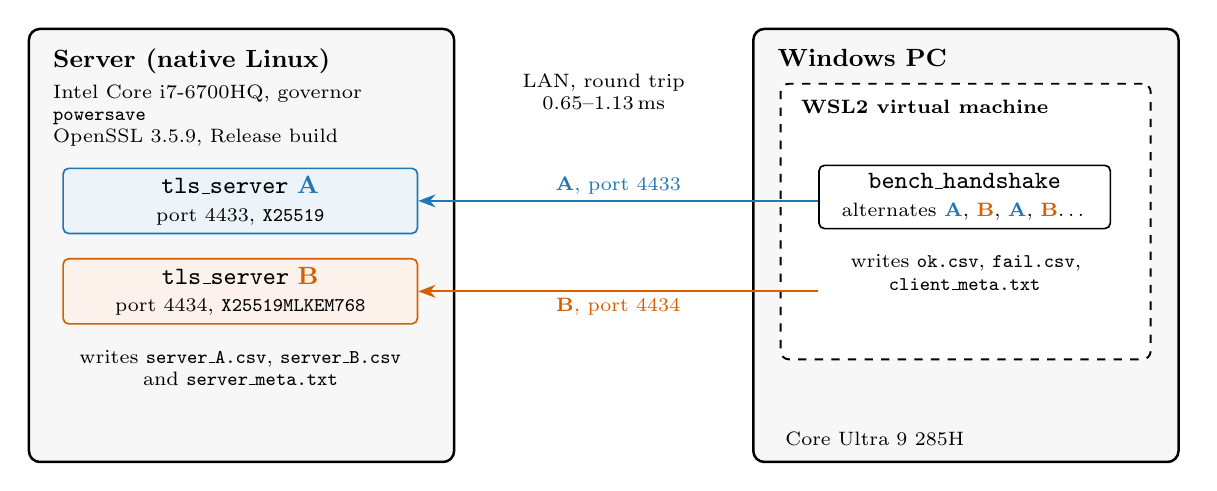
\begin{tikzpicture}[x=1cm,y=1cm]
  % server
  \node[mach, minimum width=5.4cm, minimum height=5.5cm, anchor=north west] (S) at (0,0) {};
  \node[font=\small\bfseries, anchor=north west] at ([shift={(0.2,-0.15)}]S.north west) {Server (native Linux)};
  \node[font=\scriptsize, anchor=north west, text width=4.9cm] at ([shift={(0.2,-0.6)}]S.north west)
       {Intel Core i7-6700HQ, governor \texttt{powersave}\\OpenSSL 3.5.9, Release build};
  \node[box, draw=colorA, fill=colorA!8, minimum width=4.5cm] (SA) at ([shift={(2.7,-2.2)}]S.north west)
       {\texttt{tls\_server} \cA{}\\[-1pt]\scriptsize port 4433, \texttt{X25519}};
  \node[box, draw=colorB, fill=colorB!8, minimum width=4.5cm, below=3mm of SA] (SB)
       {\texttt{tls\_server} \cB{}\\[-1pt]\scriptsize port 4434, \texttt{X25519MLKEM768}};
  \node[font=\scriptsize, below=2mm of SB, text width=4.6cm, align=center]
       {writes \texttt{server\_A.csv}, \texttt{server\_B.csv}\\and \texttt{server\_meta.txt}};
  % client
  \node[mach, minimum width=5.4cm, minimum height=5.5cm, anchor=north west] (C) at (9.2,0) {};
  \node[font=\small\bfseries, anchor=north west] at ([shift={(0.2,-0.15)}]C.north west) {Windows PC};
  \node[vm, minimum width=4.7cm, minimum height=3.5cm, anchor=north west] (W) at ([shift={(0.35,-0.7)}]C.north west) {};
  \node[font=\scriptsize\bfseries, anchor=north west] at ([shift={(0.15,-0.1)}]W.north west) {WSL2 virtual machine};
  \node[box, minimum width=3.7cm] (BH) at ([shift={(2.35,-1.45)}]W.north west)
       {\texttt{bench\_handshake}\\[-1pt]\scriptsize alternates \cA{}, \cB{}, \cA{}, \cB{}\ldots};
  \node[font=\scriptsize, below=2mm of BH, text width=3.9cm, align=center]
       {writes \texttt{ok.csv}, \texttt{fail.csv},\\\texttt{client\_meta.txt}};
  \node[font=\scriptsize, anchor=south west, text width=5cm] at ([shift={(0.3,0.1)}]C.south west) {Core Ultra 9 285H};
  % network
  \draw[arr, colorA] (BH.west |- SA.east) -- node[lbl, above=1pt] {\cA{}, port 4433} (SA.east);
  \draw[arr, colorB] ($(BH.west |- SB.east)+(0,0)$) -- node[lbl, below=1pt] {\cB{}, port 4434} (SB.east);
  \node[lbl, text width=3cm, align=center] at ($(S.east)!0.5!(C.west)+(0,1.95)$)
       {LAN, round trip\\0.65--1.13\,ms};
\end{tikzpicture}
\caption{The two machines. The client connects out to the server (solid arrows). The only files
that travel between them are the certificate authority's public certificate (once, by \texttt{scp},
fingerprint compared on both sides) and, after a session, the server's result files. Private keys
never leave the server.}
\label{fig:setup}
\end{figure}

\begin{table}[!htbp]
\centering
\begin{tabularx}{\linewidth}{@{}lX@{}}
\toprule
\textbf{Item} & \textbf{Value}\\
\midrule
Server & native Linux, \SrvCpuModel{}, CPU governor \texttt{\SrvGov}\\
Client & \CliCpuModel{} under WSL2 (a virtual machine; no governor is visible, \texttt{\CliGov})\\
Network & one LAN, no loss or delay added; \texttt{ping} round trips (min/avg/max/deviation):
  \RttOne{} (session 1), \RttTwo{} (2), \RttThree{} (3)\\
Software & OpenSSL 3.5.9, Release build, both ends; session 1 commit \texttt{\CommitOne}, sessions 2 and 3
  \texttt{\CommitTwo} / \texttt{\CommitThree}; working tree clean, same commit on both machines
  (\SameCommitOne{}/\SameCommitTwo{}/\SameCommitThree{})\\
TLS &  1.3 only, \texttt{TLS\_AES\_128\_GCM\_SHA256}, group pinned on both ends; ECDSA P-256 demo
  certificates\\
Experiment & \NOneA{} measured handshakes per configuration per session after \NWarm{} warm-up,
  \cA{} and \cB{} interleaved, a new TCP connection and a full handshake every time (no resumption)\\
Date (UTC) & \Dates{}, all three sessions\\
\bottomrule
\end{tabularx}
\caption{Conditions. They are recorded by the scripts next to every run, not typed afterwards.}
\label{tab:cond}
\end{table}

\section{How a session runs, and when it counts}

Each session uses a new run identifier, the same on both machines, so results never overwrite each
other. The order matters: the server must be started first and must be the only one.

\begin{figure}[!htbp]
\centering
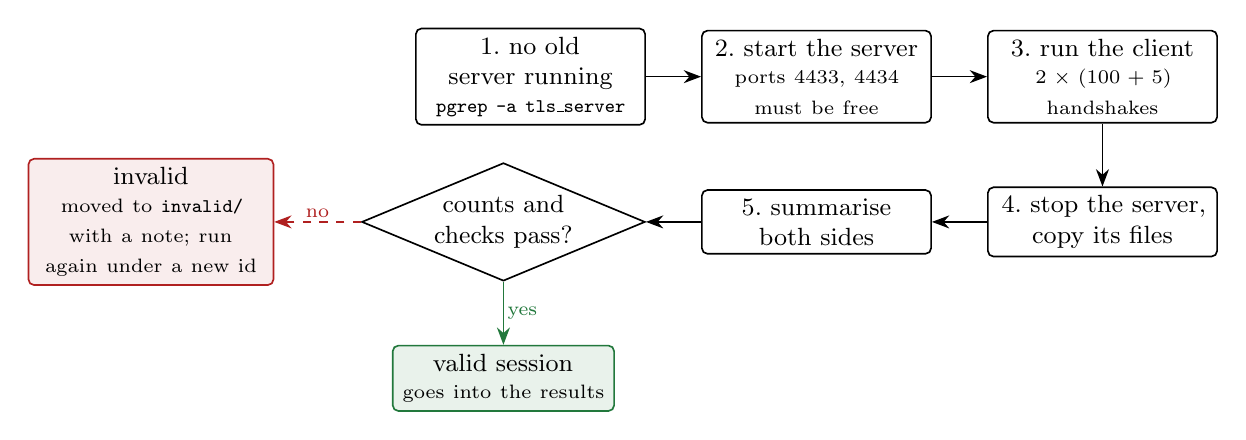
\begin{tikzpicture}[node distance=5mm and 7mm]
  \node[box, text width=2.7cm] (n1) {1.\ no old server running\\[-1pt]\scriptsize \texttt{pgrep -a tls\_server}};
  \node[box, text width=2.7cm, right=of n1] (n2) {2.\ start the server\\[-1pt]\scriptsize ports 4433, 4434 must be free};
  \node[box, text width=2.7cm, right=of n2] (n3) {3.\ run the client\\[-1pt]\scriptsize \(2\times(100+\NWarm)\) handshakes};
  \node[box, text width=2.7cm, below=8mm of n3] (n4) {4.\ stop the server, copy its files};
  \node[box, text width=2.7cm, left=of n4] (n5) {5.\ summarise both sides};
  \node[dec, left=7mm of n5] (d) {counts and\\checks pass?};
  \node[good, below=8mm of d, text width=2.6cm] (ok) {valid session\\[-1pt]\scriptsize goes into the results};
  \node[bad, left=of d, text width=2.9cm, xshift=-4mm] (no) {invalid\\[-1pt]\scriptsize moved to \texttt{invalid/} with a note; run again under a new id};
  \draw[arr] (n1) -- (n2); \draw[arr] (n2) -- (n3); \draw[arr] (n3) -- (n4);
  \draw[arr] (n4) -- (n5); \draw[arr] (n5) -- (d);
  \draw[arr, okgreen] (d) -- node[lbl, right] {yes} (ok);
  \draw[badarr] (d) -- node[lbl, above] {no} (no);
\end{tikzpicture}
\caption{One benchmark session. Step~5 is the check: a session is valid only if each configuration
shows 100 measured handshakes and no failures on both the client and the server side, the byte counts
agree (what the client sent is what the server received), and the summary prints no warning.}
\label{fig:session}
\end{figure}

The server records its own view of every handshake, so a session is a cross-check of two
independent records. This is what caught the two invalid sessions (Section~\ref{sec:invalid}).

\clearpage
\section{Results}

\FloatBarrier
\subsection{Handshake time}

Figure~\ref{fig:tls} shows the time of the TLS handshake alone, measured by the client. Every
session has the same shape: \cB{} sits above \cA{} by a small, stable amount, and the spread of each
is a few tenths of a millisecond.

\begin{figure}[!htbp]
\centering
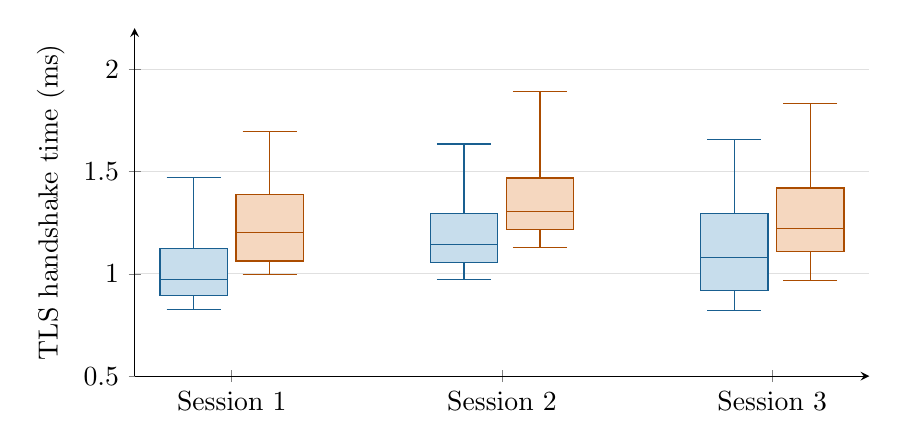
\begin{tikzpicture}
\begin{axis}[boxplot/draw direction=y, width=0.9\linewidth, height=6cm,
    ylabel={TLS handshake time (ms)}, ymin=0.5, ymax=2.2,
    xtick={1.45,4.65,7.85}, xticklabels={Session 1, Session 2, Session 3},
    axis lines=left, ymajorgrids, grid style={black!12}, xmin=0.3, xmax=9.0]
  % Generated by prepare_data3.py. Do not edit.
\addplot+[boxplot prepared={draw position=1.0, lower whisker=0.8261, lower quartile=0.8931, median=0.9713, upper quartile=1.1238, upper whisker=1.4718}, solid, fill=colorA!25, draw=colorA!80!black] coordinates {};
\addplot+[boxplot prepared={draw position=1.9, lower whisker=0.9975, lower quartile=1.0624, median=1.2027, upper quartile=1.3888, upper whisker=1.6957}, solid, fill=colorB!25, draw=colorB!80!black] coordinates {};
\addplot+[boxplot prepared={draw position=4.2, lower whisker=0.9742, lower quartile=1.0535, median=1.1418, upper quartile=1.2946, upper whisker=1.6343}, solid, fill=colorA!25, draw=colorA!80!black] coordinates {};
\addplot+[boxplot prepared={draw position=5.1, lower whisker=1.1301, lower quartile=1.2159, median=1.3047, upper quartile=1.4682, upper whisker=1.8904}, solid, fill=colorB!25, draw=colorB!80!black] coordinates {};
\addplot+[boxplot prepared={draw position=7.4, lower whisker=0.8217, lower quartile=0.9166, median=1.0798, upper quartile=1.2951, upper whisker=1.6582}, solid, fill=colorA!25, draw=colorA!80!black] coordinates {};
\addplot+[boxplot prepared={draw position=8.3, lower whisker=0.9676, lower quartile=1.1091, median=1.2198, upper quartile=1.4194, upper whisker=1.8335}, solid, fill=colorB!25, draw=colorB!80!black] coordinates {};

\end{axis}
\end{tikzpicture}
\caption{Client-measured time of the TLS handshake, \cA{} (blue) and \cB{} (orange), 100 per
box. Box: quartiles and median; whiskers: 5th and 95th percentile. Connection setup is not
included.}
\label{fig:tls}
\end{figure}

\begin{table}[!htbp]
\centering
\begin{tabular}{@{}cl rrr rrr@{}}
\toprule
 & & \multicolumn{3}{c}{TLS handshake (ms, median)} & \multicolumn{3}{c}{Server CPU (ms, median)}\\
\cmidrule(lr){3-5}\cmidrule(l){6-8}
\# & Session & \cA{} & \cB{} & B/A & \cA{} & \cB{} & B/A\\
\midrule
1 & s1 & 0.971 & 1.203 & 1.24 & 0.379 & 0.479 & 1.26\\
2 & s2b & 1.142 & 1.305 & 1.14 & 0.479 & 0.587 & 1.22\\
3 & s3b & 1.080 & 1.220 & 1.13 & 0.377 & 0.465 & 1.23
\\
\bottomrule
\end{tabular}
\caption{Medians per session. B/A is the ratio of the two medians.}
\label{tab:sess}
\end{table}

\subsection{Processor time on each end}

The hybrid handshake costs more processor time on both ends. The client's own CPU time, as measured
over the whole connect-and-handshake, rises by a factor of \CCpuRatioOne{}, \CCpuRatioTwo{} and
\CCpuRatioThree{} in the three sessions; the server's by \SCpuRatioOne{}, \SCpuRatioTwo{} and
\SCpuRatioThree{}. In absolute terms the added work per handshake is \CCpuDiffTwo{} to \CCpuDiffOne{}\,ms on the
client and \SCpuDiffThree{} to \SCpuDiffTwo{}\,ms on the server.

\begin{figure}[!htbp]
\centering
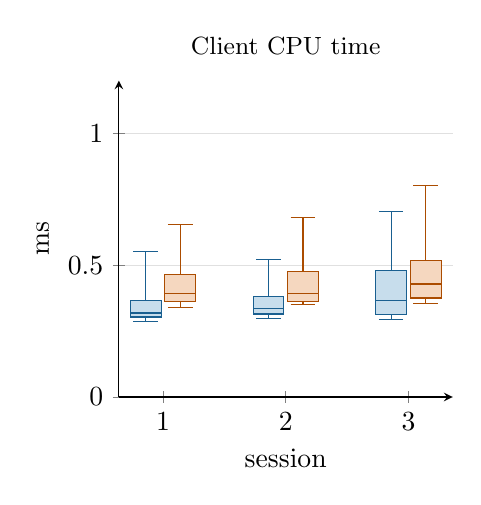
\begin{tikzpicture}
\begin{axis}[boxplot/draw direction=y, width=0.48\linewidth, height=5.6cm,
    title={\small Client CPU time}, ylabel={ms}, ymin=0, ymax=1.2,
    xtick={1.45,4.65,7.85}, xticklabels={1,2,3}, xlabel={session},
    axis lines=left, ymajorgrids, grid style={black!12}, xmin=0.3, xmax=9.0]
  % Generated by prepare_data3.py. Do not edit.
\addplot+[boxplot prepared={draw position=1.0, lower whisker=0.2876, lower quartile=0.3035, median=0.3186, upper quartile=0.3646, upper whisker=0.5525}, solid, fill=colorA!25, draw=colorA!80!black] coordinates {};
\addplot+[boxplot prepared={draw position=1.9, lower whisker=0.3393, lower quartile=0.3626, median=0.3928, upper quartile=0.4636, upper whisker=0.6529}, solid, fill=colorB!25, draw=colorB!80!black] coordinates {};
\addplot+[boxplot prepared={draw position=4.2, lower whisker=0.2980, lower quartile=0.3148, median=0.3361, upper quartile=0.3811, upper whisker=0.5204}, solid, fill=colorA!25, draw=colorA!80!black] coordinates {};
\addplot+[boxplot prepared={draw position=5.1, lower whisker=0.3523, lower quartile=0.3638, median=0.3916, upper quartile=0.4744, upper whisker=0.6818}, solid, fill=colorB!25, draw=colorB!80!black] coordinates {};
\addplot+[boxplot prepared={draw position=7.4, lower whisker=0.2927, lower quartile=0.3120, median=0.3663, upper quartile=0.4781, upper whisker=0.7033}, solid, fill=colorA!25, draw=colorA!80!black] coordinates {};
\addplot+[boxplot prepared={draw position=8.3, lower whisker=0.3539, lower quartile=0.3754, median=0.4285, upper quartile=0.5161, upper whisker=0.8021}, solid, fill=colorB!25, draw=colorB!80!black] coordinates {};

\end{axis}
\end{tikzpicture}\hfill
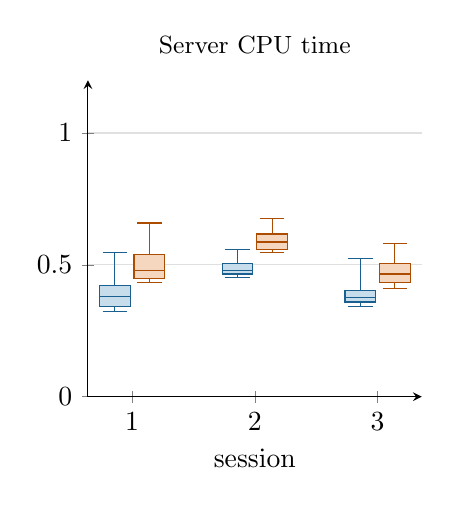
\begin{tikzpicture}
\begin{axis}[boxplot/draw direction=y, width=0.48\linewidth, height=5.6cm,
    title={\small Server CPU time}, ymin=0, ymax=1.2,
    xtick={1.45,4.65,7.85}, xticklabels={1,2,3}, xlabel={session},
    axis lines=left, ymajorgrids, grid style={black!12}, xmin=0.3, xmax=9.0]
  % Generated by prepare_data3.py. Do not edit.
\addplot+[boxplot prepared={draw position=1.0, lower whisker=0.3236, lower quartile=0.3435, median=0.3789, upper quartile=0.4221, upper whisker=0.5483}, solid, fill=colorA!25, draw=colorA!80!black] coordinates {};
\addplot+[boxplot prepared={draw position=1.9, lower whisker=0.4315, lower quartile=0.4479, median=0.4787, upper quartile=0.5406, upper whisker=0.6587}, solid, fill=colorB!25, draw=colorB!80!black] coordinates {};
\addplot+[boxplot prepared={draw position=4.2, lower whisker=0.4534, lower quartile=0.4653, median=0.4795, upper quartile=0.5044, upper whisker=0.5593}, solid, fill=colorA!25, draw=colorA!80!black] coordinates {};
\addplot+[boxplot prepared={draw position=5.1, lower whisker=0.5476, lower quartile=0.5594, median=0.5866, upper quartile=0.6171, upper whisker=0.6748}, solid, fill=colorB!25, draw=colorB!80!black] coordinates {};
\addplot+[boxplot prepared={draw position=7.4, lower whisker=0.3423, lower quartile=0.3591, median=0.3770, upper quartile=0.4019, upper whisker=0.5238}, solid, fill=colorA!25, draw=colorA!80!black] coordinates {};
\addplot+[boxplot prepared={draw position=8.3, lower whisker=0.4098, lower quartile=0.4344, median=0.4654, upper quartile=0.5041, upper whisker=0.5800}, solid, fill=colorB!25, draw=colorB!80!black] coordinates {};

\end{axis}
\end{tikzpicture}
\caption{CPU time of one handshake on each end, \cA{} (blue) and \cB{} (orange). The server runs
the slower processor and shows the larger absolute cost.}
\label{fig:cpu}
\end{figure}

\subsection{Why we quote ratios}

The absolute times are not stable between sessions. The server's \cA{} median is \SCpuMedOneA{},
\SCpuMedTwoA{} and \SCpuMedThreeA{}\,ms in the three sessions, a spread of about a quarter, although
nothing in the software changed and the machines were meant to be idle. The server runs the
\texttt{powersave} governor and the client is a virtual machine, so processor frequency and host
scheduling are plausible causes; we did not test which. The ratio of \cB{} to \cA{}, which both
configurations share within a session, moves far less (Figure~\ref{fig:ratio}).

\begin{figure}[!htbp]
\centering
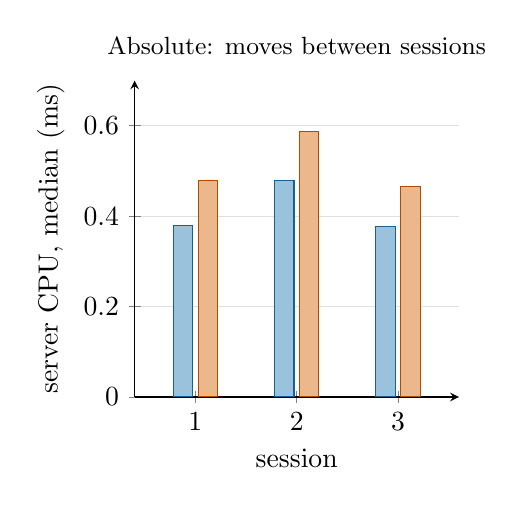
\begin{tikzpicture}
\begin{axis}[ybar, width=0.47\linewidth, height=5.6cm, bar width=7pt, ymin=0, ymax=0.7,
    ylabel={server CPU, median (ms)}, symbolic x coords={1,2,3}, xtick=data, xlabel={session},
    title={\small Absolute: moves between sessions},
    axis lines=left, ymajorgrids, grid style={black!12}, enlarge x limits=0.3]
  \addplot+[fill=colorA!45, draw=colorA!80!black] coordinates {(1,\SCpuMedOneA) (2,\SCpuMedTwoA) (3,\SCpuMedThreeA)};
  \addplot+[fill=colorB!45, draw=colorB!80!black] coordinates {(1,\SCpuMedOneB) (2,\SCpuMedTwoB) (3,\SCpuMedThreeB)};
\end{axis}
\end{tikzpicture}\hfill
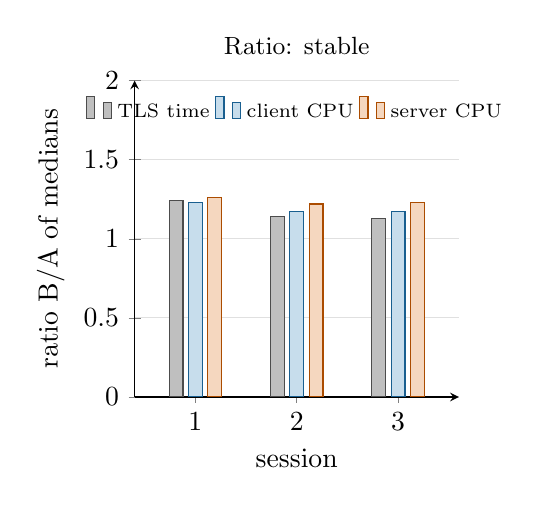
\begin{tikzpicture}
\begin{axis}[ybar, width=0.47\linewidth, height=5.6cm, bar width=5pt, ymin=0, ymax=2.0,
    ylabel={ratio B/A of medians}, symbolic x coords={1,2,3}, xtick=data, xlabel={session},
    title={\small Ratio: stable},
    axis lines=left, ymajorgrids, grid style={black!12}, enlarge x limits=0.3,
    legend style={font=\scriptsize, at={(0.5,0.97)}, anchor=north, legend columns=-1, draw=none, fill=none}]
  \addplot+[fill=black!25, draw=black!70] coordinates {(1,\TlsRatioOne) (2,\TlsRatioTwo) (3,\TlsRatioThree)};
  \addplot+[fill=colorA!25, draw=colorA!80!black] coordinates {(1,\CCpuRatioOne) (2,\CCpuRatioTwo) (3,\CCpuRatioThree)};
  \addplot+[fill=colorB!25, draw=colorB!80!black] coordinates {(1,\SCpuRatioOne) (2,\SCpuRatioTwo) (3,\SCpuRatioThree)};
  \legend{TLS time, client CPU, server CPU}
\end{axis}
\end{tikzpicture}
\caption{Left: the server's CPU time moves by a quarter from session to session (\cA{} blue, \cB{} orange).
Right: the ratio of \cB{} to \cA{} for the handshake time, client CPU and server CPU.}
\label{fig:ratio}
\end{figure}

\subsection{Bytes and memory}

Message sizes and memory are deterministic, not statistical: they were the same in all three sessions.
Both ends agree on the bytes in every handshake (what one sent, the other received).

\begin{table}[!htbp]
\centering
\begin{tabular}{@{}l rr r@{}}
\toprule
 & \cA{} & \cB{} & Difference\\
\midrule
Client sends in the handshake & \CtxA{} & \CtxB{} & +1{,}176\\
Client receives & \CrxA{} & \CrxB{} & +1{,}088\\
Heap held by an open connection, client & \ChA{} & \ChB{} & +7{,}888\\
Heap held by an open connection, server & \ShA{} & \ShB{} & +6{,}064\\
\bottomrule
\end{tabular}
\caption{Per handshake, median. The byte differences equal those measured on loopback (Report~2 and \texttt{results.md}). The
client's extra 1{,}176 bytes are 8 fewer than the 1{,}184-byte key it sends; we have not explained the 8.}
\label{tab:bytes}
\end{table}

\section{The slow connects in configuration B}
\label{sec:slow}

Figure~\ref{fig:scatter} plots every measured attempt. Almost all sit within a few milliseconds.
But in every session, exactly two attempts of configuration~\cB{} took about one second from
\texttt{connect()} to the end of the handshake (\NSlow{} of the 600 \cB{} attempts, none of \cA{}).

\begin{figure}[!htbp]
\centering
\begin{tikzpicture}
  \scatterpanel{One}{1}{1.2cm}{ylabel={connect to handshake end (ms)}}
  \scatterpanel{Two}{2}{6.5cm}{}
  \scatterpanel{Three}{3}{11.8cm}{}
\end{tikzpicture}
\caption{Time from \texttt{connect()} to the end of the handshake for every measured attempt, on a
logarithmic axis (\cA{} blue, \cB{} orange). The attempts alternate \cA{}, \cB{}, so the two colours
interleave along the horizontal axis; the warm-up attempts are not plotted.}
\label{fig:scatter}
\end{figure}

\begin{table}[!htbp]
\centering
\begin{tabular}{@{}ccrrr@{}}
\toprule
Session & Config & Attempt & Connect to end (ms) & TLS part (ms)\\
\midrule
1 & B & 59 & 1018 & 2.4\\
1 & B & 163 & 1018 & 1.7\\
2 & B & 97 & 1023 & 2.0\\
2 & B & 197 & 1015 & 1.5\\
3 & B & 97 & 1031 & 2.2\\
3 & B & 197 & 1029 & 2.2
\\
\bottomrule
\end{tabular}
\caption{The attempts that took longer than 100\,ms. The TLS part of the same attempts was normal.}
\label{tab:slow}
\end{table}

What the data show: the time was spent \emph{before} the TLS handshake started
(\SlowTlsMax{}\,ms at most for the TLS part, \SlowMin{} to \SlowMax{}\,ms in total). About one second
is the usual wait before a TCP connection attempt is retried after a lost first packet. So a
connection attempt to the \cB{} server's port was lost and repeated. It does not move the median or
the 95th percentile (2 of 100 is below 5 percent), but it would raise a mean or a maximum.

What we do not know: why it only affects \cB{}, why it comes twice in every session, and where the
packet was lost. We did not capture the traffic, because this run is a proof of concept for the
procedure and the real test is on the Raspberry~Pis. \textbf{This is not evidence that the hybrid
group makes connections slower}; the TLS part of those attempts is as fast as the others.

\section{Two sessions we threw away}
\label{sec:invalid}

The first attempts at sessions~2 and~3 were invalid. The check in Figure~\ref{fig:session} caught
them: the first stopped agreeing with itself, and the second had nothing to summarise.

\begin{figure}[!htbp]
\centering
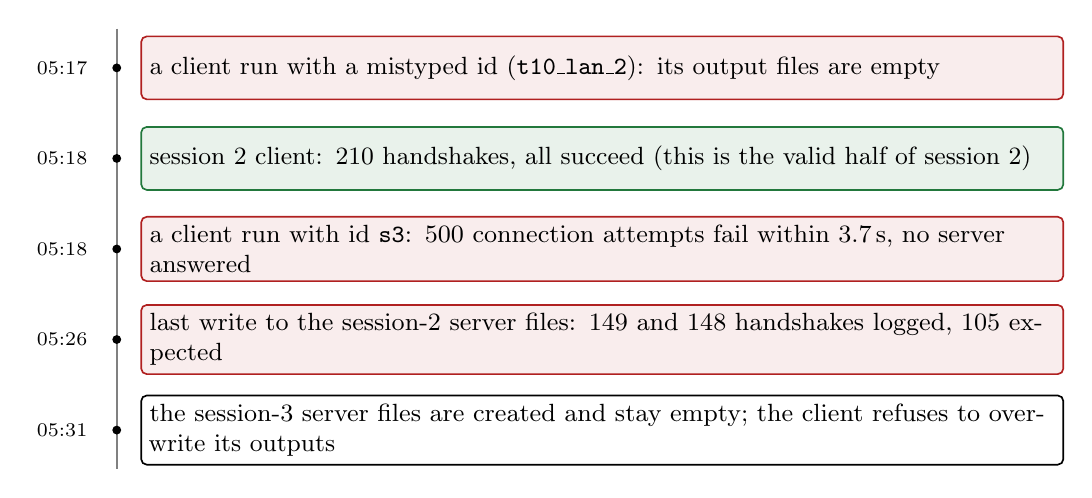
\begin{tikzpicture}[node distance=3mm]
  \node[font=\scriptsize, anchor=east] (t1) at (0,0) {05:17};
  \node[font=\scriptsize, anchor=east] (t2) at (0,-1.15) {05:18};
  \node[font=\scriptsize, anchor=east] (t3) at (0,-2.3) {05:18};
  \node[font=\scriptsize, anchor=east] (t4) at (0,-3.45) {05:26};
  \node[font=\scriptsize, anchor=east] (t5) at (0,-4.6) {05:31};
  \draw[line width=0.6pt, black!50] (0.25,0.5) -- (0.25,-5.1);
  \foreach \y in {0,-1.15,-2.3,-3.45,-4.6} {\fill (0.25,\y) circle (1.6pt);}
  \node[bad, anchor=west, text width=11.5cm, align=left] at (0.55,0)
       {a client run with a mistyped id (\texttt{t10\_lan\_2}): its output files are empty};
  \node[good, anchor=west, text width=11.5cm, align=left] at (0.55,-1.15)
       {session 2 client: 210 handshakes, all succeed (this is the valid half of session 2)};
  \node[bad, anchor=west, text width=11.5cm, align=left] at (0.55,-2.3)
       {a client run with id \texttt{s3}: 500 connection attempts fail within 3.7\,s, no server answered};
  \node[bad, anchor=west, text width=11.5cm, align=left] at (0.55,-3.45)
       {last write to the session-2 server files: 149 and 148 handshakes logged, 105 expected};
  \node[box, anchor=west, text width=11.5cm, align=left] at (0.55,-4.6)
       {the session-3 server files are created and stay empty; the client refuses to overwrite its outputs};
\end{tikzpicture}
\caption{What the files show for the two invalid sessions, in order of their time stamps (UTC, minutes
past 05:00 on 2026-10-20). Which client run reached the old servers is not recorded.}
\label{fig:invalid}
\end{figure}

The facts: the session-2 server files held 149 and 148 handshakes where the client made 105, and
were last written about eight minutes after the client finished, so some other client had connected
to servers that should have been stopped. A client started under the next identifier found no server and
failed all 500 attempts in under four seconds. The later server run recorded no handshakes. Servers left running from a
test run were also found on the server machine; they listen on other ports and did not cause this,
but they show how easily a forgotten process is left behind.

We moved all of it into a folder named \texttt{invalid} with a note, did not edit any file, and
reran both sessions under new identifiers. Two changes make this harder to repeat: the server script
now refuses to start if its ports are in use, and the runbook says to check for old servers before
every session.

\section{What we claim, and what we do not}

\begin{itemize}\setlength\itemsep{0.1em}
\item \textbf{Claimed.} On these two computers and this network, the hybrid handshake
  (\prog{X25519MLKEM768}) costs about \TlsDiffThree{} to \TlsDiffOne{}\,ms more than the classical one
  (\prog{X25519}) and about 1.2 times the processor time on each end. It sends 1{,}176 bytes more and
  receives 1{,}088 more, and holds about 8\,kB (client) and 6\,kB (server) more memory per
  connection. The three sessions agree on this.
\item \textbf{Not claimed.} These are not Raspberry~Pi numbers and not gate evidence. The client is a
  virtual machine. The network is a wired LAN with a sub-millisecond round trip and no loss. Three
  sessions on one pair of machines show the result repeats here; they are not a statistical
  statement about other hardware. The one-second connects are unexplained.
\item \textbf{Authentication.} The certificates are classical (ECDSA P-256). The hybrid key
  establishment protects the session key against a future quantum computer; it is not post-quantum
  authentication. The link is an educational one, not flight-approved.
\end{itemize}

\section{What comes next}

\begin{itemize}\setlength\itemsep{0.1em}
\item The same procedure on the two Raspberry~Pis, with board identifiers and the instructor's
  initials; that is the evidence for T10.
\item The packet-loss test (T08) across a real network, which needs a way to impose loss on a real
  interface. The current runner works only inside a private network namespace on one machine.
\item Finish \texttt{results.md}, the advisor summary and the open questions (queue size, where
  loss is imposed on the Pis, the role of the Pico).
\item The runbook, \texttt{two\_machine\_setup.md}, lists every command used here.
\end{itemize}

\end{document}
